\chapter{Background}
\label{chap:bg}

This chapter gives the background of \betrfs~\citep{betrfs1,betrfs1tos,betrfs2,betrfs2tos,betrfs3}.
\betrfs is a file system based on write-optimized \bets.
Also, \betrfs adopts full-path indexing or relative-path indexing for locality.

Section~\ref{sec:bg:bet} introduces the underlying data structure in \betrfs,
the \bet.
The \bet is a WOD that treats writes as messages and cascades messages in
batches.
Then, Section~\ref{sec:bg:fpi} describes full-path-indexed \betrfs.
Full-path indexing keeps metadata and data under one directory close to each
other in the key space,
but makes the simple implementation of file system renames expensive.
Next, Section~\ref{sec:bg:rpi} discusses relative-path indexing,
the previous approach that taxes other operations to mitigate the rename issue
in \betrfs.
Finally, Section~\ref{sec:bg:impl} explains implementation details
in \betrfs.

\section{\bets}
\label{sec:bg:bet}

\bets~\citep{bet,betlogin} are \btrees, augmented with buffers in non-leaf
nodes.
New writes are injected as messages into the buffer of the root node of a \bet.
When a node's buffer becomes full, messages are flushed from that node's buffer
to one of its children.
If the child is a non-leaf node, messages are injected into the child's
buffer.
Otherwise, messages take effect on the leaf node.
An insert message becomes a key/value pair in the leaf node.
If there is an old/key/value pair with the same key in the leaf node,
the insert message overwrites the old/key value pair;
A delete message removes the old key/value pair with the same key in the leaf
node.
Therefore, in a \bet, leaf nodes only store key/value pairs, as in a \btree.
Because writes can be messages in non-leaf nodes, point and range queries on a
\bet must check the buffers along the root-to-leaf path,
as well as key/value pairs in leaf nodes.

\begin{figure}[t]
    \centering
    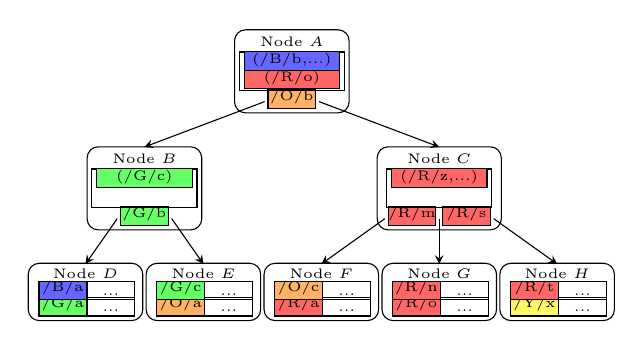
\begin{tikzpicture}[xscale=0.95, yscale=0.95]
        \node[anchor=south, rectangle, rounded corners, minimum height=.06\textwidth, minimum width=.12\textwidth, draw=black] at (0, 0) {};
        \node[anchor=south, font=\tiny] at (0, .036\textwidth) {Node $F$};
        \node[anchor=south, rectangle, minimum height=.015\textwidth, minimum width=.05\textwidth, draw=black, fill={red!60}] at (-.025\textwidth, .005\textwidth) {};
        \node[anchor=south, font=\tiny] at (-.025\textwidth, 0) {/R/a};
        \node[anchor=south, rectangle, minimum height=.015\textwidth, minimum width=.05\textwidth, draw=black] at (.028\textwidth, .005\textwidth) {};
        \node[anchor=south, font=\tiny] at (.028\textwidth, 0) {...};
        \node[anchor=south, rectangle, minimum height=.015\textwidth, minimum width=.05\textwidth, draw=black, fill={orange!60}] at (-.025\textwidth, .023\textwidth) {};
        \node[anchor=south, font=\tiny] at (-.025\textwidth, .018\textwidth) {/O/c};
        \node[anchor=south, rectangle, minimum height=.015\textwidth, minimum width=.05\textwidth, draw=black] at (.028\textwidth, .023\textwidth) {};
        \node[anchor=south, font=\tiny] at (.028\textwidth, .018\textwidth) {...};

        \node[anchor=south, rectangle, rounded corners, minimum height=.06\textwidth, minimum width=.12\textwidth, draw=black] at (.13\textwidth, 0) {};
        \node[anchor=south, font=\tiny] at (.13\textwidth, .036\textwidth) {Node $G$};
        \node[anchor=south, rectangle, minimum height=.015\textwidth, minimum width=.05\textwidth, draw=black, fill={red!60}] at (.105\textwidth, .005\textwidth) {};
        \node[anchor=south, font=\tiny] at (.105\textwidth, 0) {/R/o};
        \node[anchor=south, rectangle, minimum height=.015\textwidth, minimum width=.05\textwidth, draw=black] at (.158\textwidth, .005\textwidth) {};
        \node[anchor=south, font=\tiny] at (.158\textwidth, 0) {...};
        \node[anchor=south, rectangle, minimum height=.015\textwidth, minimum width=.05\textwidth, draw=black, fill={red!60}] at (.105\textwidth, .023\textwidth) {};
        \node[anchor=south, font=\tiny] at (.105\textwidth, .018\textwidth) {/R/n};
        \node[anchor=south, rectangle, minimum height=.015\textwidth, minimum width=.05\textwidth, draw=black] at (.158\textwidth, .023\textwidth) {};
        \node[anchor=south, font=\tiny] at (.158\textwidth, .018\textwidth) {...};

        \node[anchor=south, rectangle, rounded corners, minimum height=.06\textwidth, minimum width=.12\textwidth, draw=black] at (.26\textwidth, 0) {};
        \node[anchor=south, font=\tiny] at (.26\textwidth, .036\textwidth) {Node $H$};
        \node[anchor=south, rectangle, minimum height=.015\textwidth, minimum width=.05\textwidth, draw=black, fill={yellow!60}] at (.235\textwidth, .005\textwidth) {};
        \node[anchor=south, font=\tiny] at (.235\textwidth, 0) {/Y/x};
        \node[anchor=south, rectangle, minimum height=.015\textwidth, minimum width=.05\textwidth, draw=black] at (.288\textwidth, .005\textwidth) {};
        \node[anchor=south, font=\tiny] at (.288\textwidth, 0) {...};
        \node[anchor=south, rectangle, minimum height=.015\textwidth, minimum width=.05\textwidth, draw=black, fill={red!60}] at (.235\textwidth, .023\textwidth) {};
        \node[anchor=south, font=\tiny] at (.235\textwidth, .018\textwidth) {/R/t};
        \node[anchor=south, rectangle, minimum height=.015\textwidth, minimum width=.05\textwidth, draw=black] at (.288\textwidth, .023\textwidth) {};
        \node[anchor=south, font=\tiny] at (.288\textwidth, .018\textwidth) {...};

        \node[anchor=south, rectangle, rounded corners, minimum height=.06\textwidth, minimum width=.12\textwidth, draw=black] at (-.13\textwidth, 0) {};
        \node[anchor=south, font=\tiny] at (-.13\textwidth, .036\textwidth) {Node $E$};
        \node[anchor=south, rectangle, minimum height=.015\textwidth, minimum width=.05\textwidth, draw=black, fill={orange!60}] at (-.155\textwidth, .005\textwidth) {};
        \node[anchor=south, font=\tiny] at (-.155\textwidth, 0) {/O/a};
        \node[anchor=south, rectangle, minimum height=.015\textwidth, minimum width=.05\textwidth, draw=black] at (-.102\textwidth, .005\textwidth) {};
        \node[anchor=south, font=\tiny] at (-.102\textwidth, 0) {...};
        \node[anchor=south, rectangle, minimum height=.015\textwidth, minimum width=.05\textwidth, draw=black, fill={green!60}] at (-.155\textwidth, .023\textwidth) {};
        \node[anchor=south, font=\tiny] at (-.155\textwidth, .018\textwidth) {/G/c};
        \node[anchor=south, rectangle, minimum height=.015\textwidth, minimum width=.05\textwidth, draw=black] at (-.102\textwidth, .023\textwidth) {};
        \node[anchor=south, font=\tiny] at (-.102\textwidth, .018\textwidth) {...};

        \node[anchor=south, rectangle, rounded corners, minimum height=.06\textwidth, minimum width=.12\textwidth, draw=black] at (-.26\textwidth, 0) {};
        \node[anchor=south, font=\tiny] at (-.26\textwidth, .036\textwidth) {Node $D$};
        \node[anchor=south, rectangle, minimum height=.015\textwidth, minimum width=.05\textwidth, draw=black, fill={green!60}] at (-.285\textwidth, .005\textwidth) {};
        \node[anchor=south, font=\tiny] at (-.285\textwidth, 0) {/G/a};
        \node[anchor=south, rectangle, minimum height=.015\textwidth, minimum width=.05\textwidth, draw=black] at (-.232\textwidth, .005\textwidth) {};
        \node[anchor=south, font=\tiny] at (-.232\textwidth, 0) {...};
        \node[anchor=south, rectangle, minimum height=.015\textwidth, minimum width=.05\textwidth, draw=black, fill={blue!60}] at (-.285\textwidth, .023\textwidth) {};
        \node[anchor=south, font=\tiny] at (-.285\textwidth, .018\textwidth) {/B/a};
        \node[anchor=south, rectangle, minimum height=.015\textwidth, minimum width=.05\textwidth, draw=black] at (-.232\textwidth, .023\textwidth) {};
        \node[anchor=south, font=\tiny] at (-.232\textwidth, .018\textwidth) {...};

        \node[anchor=south, rectangle, rounded corners, minimum height=.087\textwidth, minimum width=.12\textwidth, draw=black] at (-.195\textwidth, .1\textwidth) {};
        \node[anchor=south, font=\tiny] at (-.195\textwidth, .163\textwidth) {Node $B$};
        \node[anchor=south, rectangle, minimum height=.015\textwidth, minimum width=.05\textwidth, draw=black, fill={green!60}] at (-.195\textwidth, .105\textwidth) {};
        \node[anchor=south, font=\tiny] at (-.195\textwidth, .1\textwidth) {/G/b};
        \node[anchor=south, rectangle, minimum height=.04\textwidth, minimum width=.11\textwidth, draw=black] at (-.195\textwidth, .125\textwidth) {};
        \node[anchor=south, rectangle, minimum height=.015\textwidth, minimum width=.1\textwidth, draw=black, fill={green!60}] at (-.195\textwidth, .147\textwidth) {};
        \node[anchor=south, font=\tiny] at  (-.195\textwidth, .141\textwidth) {\delm(/G/c)};

        \node[anchor=south, rectangle, rounded corners, minimum height=.087\textwidth, minimum width=.13\textwidth, draw=black] at (.13\textwidth, .1\textwidth) {};
        \node[anchor=south, font=\tiny] at (.13\textwidth, .163\textwidth) {Node $C$};
        \node[anchor=south, rectangle, minimum height=.015\textwidth, minimum width=.05\textwidth, draw=black, fill={red!60}] at (.1\textwidth, .105\textwidth) {};
        \node[anchor=south, font=\tiny] at (.1\textwidth, .1\textwidth) {/R/m};
        \node[anchor=south, rectangle, minimum height=.015\textwidth, minimum width=.05\textwidth, draw=black, fill={red!60}] at (.16\textwidth, .105\textwidth) {};
        \node[anchor=south, font=\tiny] at (.16\textwidth, .1\textwidth) {/R/s};
        \node[anchor=south, rectangle, minimum height=.04\textwidth, minimum width=.11\textwidth, draw=black] at (.13\textwidth, .125\textwidth) {};
        \node[anchor=south, rectangle, minimum height=.015\textwidth, minimum width=.1\textwidth, draw=black, fill={red!60}] at (.13\textwidth, .147\textwidth) {};
        \node[anchor=south, font=\tiny] at  (.13\textwidth, .141\textwidth) {\putm(/R/z,...)};

        \node[anchor=south, rectangle, rounded corners, minimum height=.087\textwidth, minimum width=.12\textwidth, draw=black] at (-.0325\textwidth, .229\textwidth) {};
        \node[anchor=south, font=\tiny] at (-.0325\textwidth, .292\textwidth) {Node $A$};
        \node[anchor=south, rectangle, minimum height=.015\textwidth, minimum width=.05\textwidth, draw=black, fill={orange!60}] at (-.0325\textwidth, .234\textwidth) {};
        \node[anchor=south, font=\tiny] at (-.0325\textwidth, .229\textwidth) {/O/b};
        \node[anchor=south, rectangle, minimum height=.04\textwidth, minimum width=.11\textwidth, draw=black] at (-.0325\textwidth, .254\textwidth) {};
        \node[anchor=south, rectangle, minimum height=.015\textwidth, minimum width=.1\textwidth, draw=black, fill={red!60}] at (-.0325\textwidth, .256\textwidth) {};
        \node[anchor=south, font=\tiny] at  (-.0325\textwidth, .25\textwidth) {\delm(/R/o)};
        \node[anchor=south, rectangle, minimum height=.015\textwidth, minimum width=.1\textwidth, draw=black, fill={blue!60}] at (-.0325\textwidth, .276\textwidth) {};
        \node[anchor=south, font=\tiny] at  (-.0325\textwidth, .27\textwidth) {\putm(/B/b,...)};

        \draw[->, >=stealth] (-.225\textwidth, .113\textwidth) -- (-.26\textwidth, .063\textwidth);
        \draw[->, >=stealth] (-.165\textwidth, .113\textwidth) -- (-.13\textwidth, .063\textwidth);
        \draw[->, >=stealth] (.13\textwidth, .113\textwidth) -- (.13\textwidth, .063\textwidth);
        \draw[->, >=stealth] (.19\textwidth, .113\textwidth) -- (.26\textwidth, .063\textwidth);
        \draw[->, >=stealth] (.07\textwidth, .113\textwidth) -- (0, .063\textwidth);
        \draw[->, >=stealth] (-.0625\textwidth, .242\textwidth) -- (-.195\textwidth, .192\textwidth);
        \draw[->, >=stealth] (-.0025\textwidth, .242\textwidth) -- (.13\textwidth, .192\textwidth);
    \end{tikzpicture}
    \caption[A \bet example]{\label{fig:bet}
        In a \bet, a leaf nodes stores key/value pairs, while a non-leaf node
        has pivots, parent-to-child pointers and a message buffer.}
\end{figure}

Figure~\ref{fig:bet} shows a \bet example.
Node $D$, $E$, $F$, $G$ and $H$ are leaf nodes that store key/value pairs.
Each leaf node shows key/value pairs in rows,
and each row represents a key/value pair, with the left part as the key and
the right part as the value.
We use different colors to indicate keys with different prefixes and omit the
content of the value as dots throughout the dissertation.
Node $A$, $B$ and $C$ are non-leaf nodes that contains pivots, parent-to-child
pointers and messages in buffers.
Parent-to-child pointers connect all nodes into a tree, and the left and right
pivots of a parent-to-child pointer bound the key range of the child node.
Messages in the buffers of non-leaf nodes are write operations that have been
applied to the \bet but have not taken effect on leaf nodes.
For example, the message \delm(``/G/c'') in Node $B$ indicates that the key
``/G/c'' has been deleted.
Therefore, though a query for ``/G/c'' can find the key/value pair with the
key in Node $E$,
that key/value pair is invalidated by the message in Node $B$ and the
query returns \texttt{NOT\_FOUND}.
Likewise, a query for ``/R/z'' returns the value in the message
\putm(``/R/z'',...) in node $C$.

\begin{table}[t]
    \centering
    \begin{tabular}{c | c c c}
        \hline
        Data Structure & Insert & Point Query & Range Query \\
        \hline
        \hline
        \btree & $O(log_{B}{N})$ & $O(log_{B}{N})$ & $O(log_{B}{N} + k/B)$\\
        \hline
        \bet & $O({log_{B}{N}}/{\varepsilon B^{1 - \varepsilon}})$ & $O({log_{B}{N}}/{\varepsilon})$ & $O({log_{B}{N}}/{\varepsilon} + k/B)$ \\
        \hline
        \bet ($\varepsilon=1$) & $O(log_{B}{N})$ & $O(log_{B}{N})$ & $O(log_{B}{N} + k/B)$ \\
        \hline
        \bet ($\varepsilon=0.5$) & $O(log_{B}{N}/{\sqrt{B}})$ & $O(log_{B}{N})$ & $O(log_{B}{N} + k/B)$ \\
        \hline
    \end{tabular}
    \caption[The asymptotic I/O costs of \btrees and \bets]{\label{tab:betbtree}
        The asymptotic I/O costs of \btrees and \bets.}
\end{table}

\bets are asymptotically faster than \btrees, as summarized in
Table~\ref{tab:betbtree}.
Consider a \btree with $N$ key/value pairs and in which each node can hold
$B$ keys
(for simplicity, assume keys have constant size and that the value associated
with each key has negligible size).
The tree has fanout $B$, so its height is $O(log_{B}{N})$.
Inserts and point queries need to fetch all nodes along the root-to-leaf path,
resulting in $O(log_{B}{N})$ I/Os.
A range query for $k$ key/value pairs requires $O(log_{B}{N} + k/B)$ I/Os.

For comparison, a \bet with node size $B$ has fanout $B^{\varepsilon}$, where
$0 < \varepsilon \leq 1$.
Therefore, pivot keys in a non-leaf node consume $B^{\varepsilon}$ space and
the remaining $(B - B^{\varepsilon})$ space is used for the message buffer.
As a result, the \bet has height $O(log_{B}{N}/\varepsilon)$.
A point query fetches all nodes along the root-to-leaf path,
inspecting messages in the buffers of non-leaf nodes and key/value pairs in the
leaf node.
Therefore, the total I/O cost is $O(log_{B}{N}/\varepsilon)$.
Likewise,  a range query for $k$ key/value pairs
requires $O({log_{B}{N}}/{\varepsilon} + k/B)$ I/Os.
On the other hand, the cost of an insert consists of injecting the message into
the root node with $O(1)$ I/Os and flushing the message down at each level.
In each flush, \bets has $O(B - B^{\varepsilon})$ messages and $B^{\varepsilon}$
children.
Thus, at least one child can receive no less than
$O((B - B^{\varepsilon})/B^{\varepsilon}) = O(B^{1 - \varepsilon})$ messages.
Therefore, the amortized cost of an insert in one flush is
$O(1/B^{1 - \varepsilon})$.
As the insert must be flushed $O(log_{B}{N}/\varepsilon)$ (tree height) times,
the amortized cost of the insert is
$O({log_{B}{N}}/{\varepsilon B^{1 - \varepsilon}})$.
A \bet with $\varepsilon = 1$ is equivalent to a \btree.
And if we set $\varepsilon = 1/2$, the point and range query costs of the \bet
become $O(log_{B}{N})$ and $O(log_{B}{N} + k/B)$, which is the same as a \btree,
but the insert cost becomes $O(log_{B}{N}/{\sqrt{B}})$, which is faster by a
factor of $\sqrt{B}$.

One important change in \bets from \btrees is the asymmetric I/O costs for
point queries and inserts.
If an application wants to update the old value associated with a key,
a \btree will perform a point query to get the old value and then issue an
insert with the updated value.
Because both operations take $O(log_{B}{N})$ I/Os, the total cost remains
$O(log_{B}{N})$.
However, in \bets, the query cost is $O(log_{B}{N}/\varepsilon)$ I/Os while the
insert cost is $O({log_{B}{N}}/{\varepsilon B^{1 - \varepsilon}})$.
A query for the old value degrades the update cost to
$O(log_{B}{N}/\varepsilon)$ I/Os.

To avoid this read-before-write problem, \bets introduce ``upsert'' operations.
An upsert operation injects an \upsertm message with the key and a delta into the
buffer of the root node.
When the \upsertm message is flushed to the leaf, it updates the old value
associated with the key with a user-specified function and the delta in the
message.
With the introduction of \upsertm messages,
queries need to compute the new value on the fly if \upsertm messages have not
reached the leaf node,
however, this doesn't change the I/O costs of queries.
On the other hand, updating an old value becomes as fast as an insert operation,
because it doesn't need to fetch the old value.


\begin{figure}[t]
    \centering
    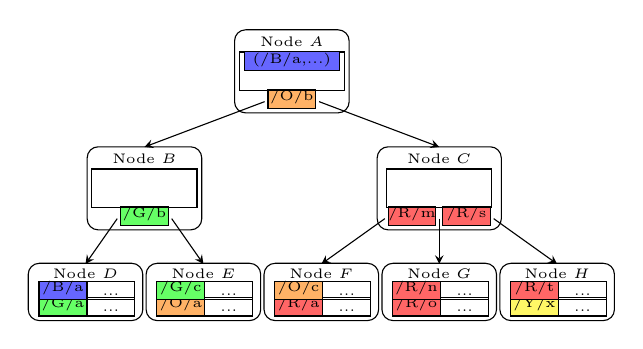
\begin{tikzpicture}[xscale=0.95, yscale=0.95]
        \node[anchor=south, rectangle, rounded corners, minimum height=.06\textwidth, minimum width=.12\textwidth, draw=black] at (0, 0) {};
        \node[anchor=south, font=\tiny] at (0, .036\textwidth) {Node $F$};
        \node[anchor=south, rectangle, minimum height=.015\textwidth, minimum width=.05\textwidth, draw=black, fill={red!60}] at (-.025\textwidth, .005\textwidth) {};
        \node[anchor=south, font=\tiny] at (-.025\textwidth, 0) {/R/a};
        \node[anchor=south, rectangle, minimum height=.015\textwidth, minimum width=.05\textwidth, draw=black] at (.028\textwidth, .005\textwidth) {};
        \node[anchor=south, font=\tiny] at (.028\textwidth, 0) {...};
        \node[anchor=south, rectangle, minimum height=.015\textwidth, minimum width=.05\textwidth, draw=black, fill={orange!60}] at (-.025\textwidth, .023\textwidth) {};
        \node[anchor=south, font=\tiny] at (-.025\textwidth, .018\textwidth) {/O/c};
        \node[anchor=south, rectangle, minimum height=.015\textwidth, minimum width=.05\textwidth, draw=black] at (.028\textwidth, .023\textwidth) {};
        \node[anchor=south, font=\tiny] at (.028\textwidth, .018\textwidth) {...};

        \node[anchor=south, rectangle, rounded corners, minimum height=.06\textwidth, minimum width=.12\textwidth, draw=black] at (.13\textwidth, 0) {};
        \node[anchor=south, font=\tiny] at (.13\textwidth, .036\textwidth) {Node $G$};
        \node[anchor=south, rectangle, minimum height=.015\textwidth, minimum width=.05\textwidth, draw=black, fill={red!60}] at (.105\textwidth, .005\textwidth) {};
        \node[anchor=south, font=\tiny] at (.105\textwidth, 0) {/R/o};
        \node[anchor=south, rectangle, minimum height=.015\textwidth, minimum width=.05\textwidth, draw=black] at (.158\textwidth, .005\textwidth) {};
        \node[anchor=south, font=\tiny] at (.158\textwidth, 0) {...};
        \node[anchor=south, rectangle, minimum height=.015\textwidth, minimum width=.05\textwidth, draw=black, fill={red!60}] at (.105\textwidth, .023\textwidth) {};
        \node[anchor=south, font=\tiny] at (.105\textwidth, .018\textwidth) {/R/n};
        \node[anchor=south, rectangle, minimum height=.015\textwidth, minimum width=.05\textwidth, draw=black] at (.158\textwidth, .023\textwidth) {};
        \node[anchor=south, font=\tiny] at (.158\textwidth, .018\textwidth) {...};

        \node[anchor=south, rectangle, rounded corners, minimum height=.06\textwidth, minimum width=.12\textwidth, draw=black] at (.26\textwidth, 0) {};
        \node[anchor=south, font=\tiny] at (.26\textwidth, .036\textwidth) {Node $H$};
        \node[anchor=south, rectangle, minimum height=.015\textwidth, minimum width=.05\textwidth, draw=black, fill={yellow!60}] at (.235\textwidth, .005\textwidth) {};
        \node[anchor=south, font=\tiny] at (.235\textwidth, 0) {/Y/x};
        \node[anchor=south, rectangle, minimum height=.015\textwidth, minimum width=.05\textwidth, draw=black] at (.288\textwidth, .005\textwidth) {};
        \node[anchor=south, font=\tiny] at (.288\textwidth, 0) {...};
        \node[anchor=south, rectangle, minimum height=.015\textwidth, minimum width=.05\textwidth, draw=black, fill={red!60}] at (.235\textwidth, .023\textwidth) {};
        \node[anchor=south, font=\tiny] at (.235\textwidth, .018\textwidth) {/R/t};
        \node[anchor=south, rectangle, minimum height=.015\textwidth, minimum width=.05\textwidth, draw=black] at (.288\textwidth, .023\textwidth) {};
        \node[anchor=south, font=\tiny] at (.288\textwidth, .018\textwidth) {...};

        \node[anchor=south, rectangle, rounded corners, minimum height=.06\textwidth, minimum width=.12\textwidth, draw=black] at (-.13\textwidth, 0) {};
        \node[anchor=south, font=\tiny] at (-.13\textwidth, .036\textwidth) {Node $E$};
        \node[anchor=south, rectangle, minimum height=.015\textwidth, minimum width=.05\textwidth, draw=black, fill={orange!60}] at (-.155\textwidth, .005\textwidth) {};
        \node[anchor=south, font=\tiny] at (-.155\textwidth, 0) {/O/a};
        \node[anchor=south, rectangle, minimum height=.015\textwidth, minimum width=.05\textwidth, draw=black] at (-.102\textwidth, .005\textwidth) {};
        \node[anchor=south, font=\tiny] at (-.102\textwidth, 0) {...};
        \node[anchor=south, rectangle, minimum height=.015\textwidth, minimum width=.05\textwidth, draw=black, fill={green!60}] at (-.155\textwidth, .023\textwidth) {};
        \node[anchor=south, font=\tiny] at (-.155\textwidth, .018\textwidth) {/G/c};
        \node[anchor=south, rectangle, minimum height=.015\textwidth, minimum width=.05\textwidth, draw=black] at (-.102\textwidth, .023\textwidth) {};
        \node[anchor=south, font=\tiny] at (-.102\textwidth, .018\textwidth) {...};

        \node[anchor=south, rectangle, rounded corners, minimum height=.06\textwidth, minimum width=.12\textwidth, draw=black] at (-.26\textwidth, 0) {};
        \node[anchor=south, font=\tiny] at (-.26\textwidth, .036\textwidth) {Node $D$};
        \node[anchor=south, rectangle, minimum height=.015\textwidth, minimum width=.05\textwidth, draw=black, fill={green!60}] at (-.285\textwidth, .005\textwidth) {};
        \node[anchor=south, font=\tiny] at (-.285\textwidth, 0) {/G/a};
        \node[anchor=south, rectangle, minimum height=.015\textwidth, minimum width=.05\textwidth, draw=black] at (-.232\textwidth, .005\textwidth) {};
        \node[anchor=south, font=\tiny] at (-.232\textwidth, 0) {...};
        \node[anchor=south, rectangle, minimum height=.015\textwidth, minimum width=.05\textwidth, draw=black, fill={blue!60}] at (-.285\textwidth, .023\textwidth) {};
        \node[anchor=south, font=\tiny] at (-.285\textwidth, .018\textwidth) {/B/a};
        \node[anchor=south, rectangle, minimum height=.015\textwidth, minimum width=.05\textwidth, draw=black] at (-.232\textwidth, .023\textwidth) {};
        \node[anchor=south, font=\tiny] at (-.232\textwidth, .018\textwidth) {...};

        \node[anchor=south, rectangle, rounded corners, minimum height=.087\textwidth, minimum width=.12\textwidth, draw=black] at (-.195\textwidth, .1\textwidth) {};
        \node[anchor=south, font=\tiny] at (-.195\textwidth, .163\textwidth) {Node $B$};
        \node[anchor=south, rectangle, minimum height=.015\textwidth, minimum width=.05\textwidth, draw=black, fill={green!60}] at (-.195\textwidth, .105\textwidth) {};
        \node[anchor=south, font=\tiny] at (-.195\textwidth, .1\textwidth) {/G/b};
        \node[anchor=south, rectangle, minimum height=.04\textwidth, minimum width=.11\textwidth, draw=black] at (-.195\textwidth, .125\textwidth) {};

        \node[anchor=south, rectangle, rounded corners, minimum height=.087\textwidth, minimum width=.13\textwidth, draw=black] at (.13\textwidth, .1\textwidth) {};
        \node[anchor=south, font=\tiny] at (.13\textwidth, .163\textwidth) {Node $C$};
        \node[anchor=south, rectangle, minimum height=.015\textwidth, minimum width=.05\textwidth, draw=black, fill={red!60}] at (.1\textwidth, .105\textwidth) {};
        \node[anchor=south, font=\tiny] at (.1\textwidth, .1\textwidth) {/R/m};
        \node[anchor=south, rectangle, minimum height=.015\textwidth, minimum width=.05\textwidth, draw=black, fill={red!60}] at (.16\textwidth, .105\textwidth) {};
        \node[anchor=south, font=\tiny] at (.16\textwidth, .1\textwidth) {/R/s};
        \node[anchor=south, rectangle, minimum height=.04\textwidth, minimum width=.11\textwidth, draw=black] at (.13\textwidth, .125\textwidth) {};

        \node[anchor=south, rectangle, rounded corners, minimum height=.087\textwidth, minimum width=.12\textwidth, draw=black] at (-.0325\textwidth, .229\textwidth) {};
        \node[anchor=south, font=\tiny] at (-.0325\textwidth, .292\textwidth) {Node $A$};
        \node[anchor=south, rectangle, minimum height=.015\textwidth, minimum width=.05\textwidth, draw=black, fill={orange!60}] at (-.0325\textwidth, .234\textwidth) {};
        \node[anchor=south, font=\tiny] at (-.0325\textwidth, .229\textwidth) {/O/b};
        \node[anchor=south, rectangle, minimum height=.04\textwidth, minimum width=.11\textwidth, draw=black] at (-.0325\textwidth, .254\textwidth) {};
        \node[anchor=south, rectangle, minimum height=.015\textwidth, minimum width=.1\textwidth, draw=black, fill={blue!60}] at (-.0325\textwidth, .276\textwidth) {};
        \node[anchor=south, font=\tiny] at  (-.0325\textwidth, .27\textwidth) {\upsertm(/B/a,...)};

        \draw[->, >=stealth] (-.225\textwidth, .113\textwidth) -- (-.26\textwidth, .063\textwidth);
        \draw[->, >=stealth] (-.165\textwidth, .113\textwidth) -- (-.13\textwidth, .063\textwidth);
        \draw[->, >=stealth] (.13\textwidth, .113\textwidth) -- (.13\textwidth, .063\textwidth);
        \draw[->, >=stealth] (.19\textwidth, .113\textwidth) -- (.26\textwidth, .063\textwidth);
        \draw[->, >=stealth] (.07\textwidth, .113\textwidth) -- (0, .063\textwidth);
        \draw[->, >=stealth] (-.0625\textwidth, .242\textwidth) -- (-.195\textwidth, .192\textwidth);
        \draw[->, >=stealth] (-.0025\textwidth, .242\textwidth) -- (.13\textwidth, .192\textwidth);
    \end{tikzpicture}
    \caption[An example of an upsert in a \bet]{\label{fig:upsert}
        An upsert message stores the description of modification on the old
        value associated with the key.}
\end{figure}

Figure~\ref{fig:upsert} shows an example of an \upsertm message in the \bet.
In the example, the application wants to update the value associated with
the key ``/B/a''.
Instead of querying the \bet for the old value and then inserting the new value,
the application calls the upsert operation that injects an \upsertm message into
the root node, Node $A$.
Assume the old value associated with the key ``/B/a'' in Node $D$ is $v$,
the delta in the \upsertm message is $\Delta$,
and the user-specified function is $f$.
The \upsertm message essentially updates the value associated with the key
``/B/a'' to $f(v,\Delta)$.
Queries for the key ``/B/a'' need to calculate $f(v,\Delta)$ on the fly.
And the \upsertm message will update the value associated with the key ``/B/a''
to $f(v,\Delta)$ when the \bet flushes the message to Node $D$.

\section{Full-path-indexed \betrfs}
\label{sec:bg:fpi}

\begin{figure}[t]
    \centering
    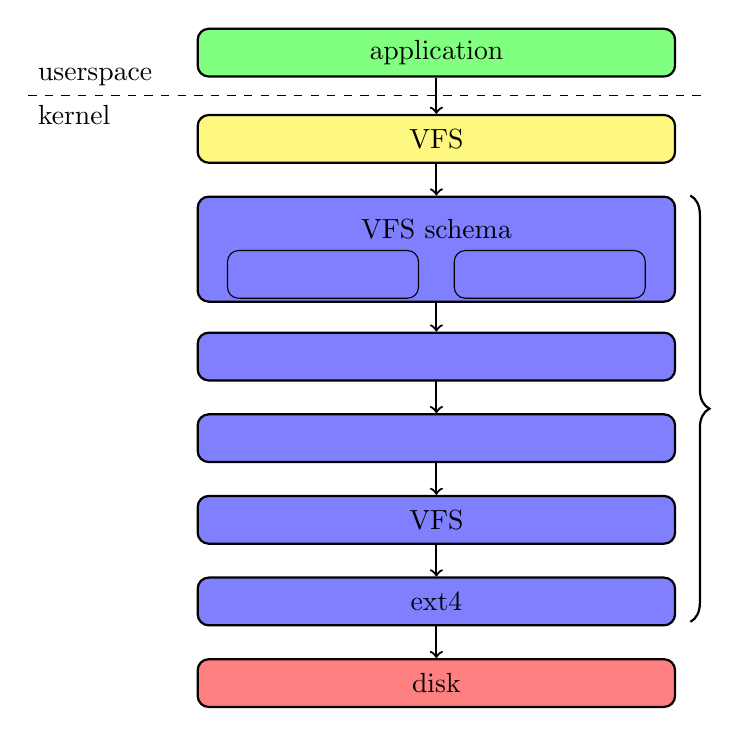
\begin{tikzpicture}[yscale=0.95, xscale=0.95]
    \draw[thick, ->] (0, .04\textwidth) -- (0, 0) node [anchor=north, rectangle, rounded corners, text centered, minimum height=.05\textwidth, minimum width=.5\textwidth, draw=black, fill=red!50] {disk};
    \draw[thick, ->] (0, .13\textwidth) -- (0, .09\textwidth) node [anchor=north, rectangle, rounded corners, text centered, minimum height=.05\textwidth, minimum width=.5\textwidth, draw=black, fill=blue!50] {ext4};
    \draw[thick, ->] (0, .22\textwidth) -- (0, .18\textwidth) node [anchor=north, rectangle, rounded corners, text centered, minimum height=.05\textwidth, minimum width=.5\textwidth, draw=black, fill=blue!50] {VFS};
    \draw[thick, ->] (0, .31\textwidth) -- (0, .27\textwidth) node [anchor=north, rectangle, rounded corners, text centered, minimum height=.05\textwidth, minimum width=.5\textwidth, draw=black, fill=blue!50] {\klibc};
    \draw[thick, ->] (0, .4\textwidth) -- (0, .36\textwidth) node [anchor=north, rectangle, rounded corners, text centered, minimum height=.05\textwidth, minimum width=.5\textwidth, draw=black, fill=blue!50] {\fti};
    \draw[thick, ->] (0, .55\textwidth) -- (0, .51\textwidth) node [anchor=north, rectangle, rounded corners, text centered, minimum height=.11\textwidth, minimum width=.5\textwidth, draw=black, fill=blue!50] {};
    \node [anchor=north, rectangle, rounded corners, text centered, minimum height=.05\textwidth, minimum width=.2\textwidth, draw=black, fill=blue!50] at (.125\textwidth, .45\textwidth) {\ddb};
    \node [anchor=north, rectangle, rounded corners, text centered, minimum height=.05\textwidth, minimum width=.2\textwidth, draw=black, fill=blue!50] at (-.125\textwidth, .45\textwidth) {\mdb};
    \node [anchor=north, text centered, minimum height=.05\textwidth] at (0, .50\textwidth) {\betrfs VFS schema};
    \draw[thick, ->] (0, .64\textwidth) -- (0, .60\textwidth) node [anchor=north, rectangle, rounded corners, text centered, minimum height=.05\textwidth, minimum width=.5\textwidth, draw=black, fill=yellow!50] {VFS};
    \node[anchor=south, rectangle, rounded corners, text centered, minimum height=.05\textwidth, minimum width=.5\textwidth, draw=black, thick, fill=green!50] at (0, .64\textwidth) {application};
    \draw[dashed] (-.45\textwidth, .62\textwidth) -- (.3\textwidth, .62\textwidth);
    \node[anchor=south west] at (-.45\textwidth, .62\textwidth) {userspace};
    \node[anchor=north west] at (-.45\textwidth, .62\textwidth) {kernel};
    \draw[decorate, decoration={brace,amplitude=.02\textwidth,mirror}, thick] (.28\textwidth, .04\textwidth) -- (.28\textwidth, .51\textwidth);
    \node[anchor=west,text centered] at (.3\textwidth, .275\textwidth) {\betrfs};
    \end{tikzpicture}
    \caption[The \betrfs architecture]{\label{fig:betrfs}
        The \betrfs architecture.}
\end{figure}

\betrfs~\citep{betrfs1,betrfs1tos} is a Linux in-kernel, full-path-indexed,
write-optimized file system built upon \fti~\citep{fti},
a key/value store that implements \bets and
exposes a key/value interface similar to Berkeley DB.

Figure~\ref{fig:betrfs} shows the \betrfs architecture.
In Linux, applications interact with file systems through system calls,
which invoke the corresponding VFS (Virtual File System) functions.
The VFS function then calls the particular function implemented by
the underlying file system.
\betrfs implements file systems operations by translating them into key/value
store operations in \fti.
\betrfs interacts with \fti through point operations, such as \texttt{put},
\texttt{get} and \texttt{del}, as well as range queries with cursors
(\texttt{c\_get} with DB\_SET\_RANGE and DB\_NEXT).
\betrfs also uses the transaction interface of \fti to execute multiple
operations atomically in one transaction.
A redo log and periodic checkpoints (every 60 seconds) in \fti ensure that
changes are made persistent on the disk.

\Fti cannot be integrated into a Linux kernel module easily because
it is a userspace library that assumes libc functions and system calls.
To address this issue, we built a shim layer called \klibc in \betrfs.
\Klibc implements all functions \fti requires.
For example, \fti requires a underlying file system to perform file operations.
To this end, \klibc privately mounts an ext4 file system and calls the
corresponding VFS functions when \fti invokes file system operations.
Through a shim layer, \betrfs can incorporate \fti into the kernel module
without modifying code in \fti.

\betrfs uses two key/value indexes to store metadata and data in the file
system.
One index, \mdb, stores metadata, mapping full-paths to \texttt{struct stat}
structures.
The other index, \ddb, stores data, mapping (full-path and block number) to
4KiB blocks.
When the file system function needs metadata, \betrfs queries
the \mdb with the full-path key and constructs the corresponding inode
from the \texttt{struct stat}.
Likewise, when a dirty inode needs to be written, the \texttt{struct stat} is
assembled from the inode and written to the \mdb with the
full-path key.
Blocks of a file are fetched and written by the full-path and the indexes of
blocks.
Although other block granularity is possible (we tried 512B for the preliminary
implementation of \betrfs), 4KiB is the natural block size
because it is the same as the page size in the Linux page cache.

\betrfs can write to a block without fetching the old block to memory, avoiding
expensive read-before-write described in Section~\ref{sec:bg:bet}.
Conventional file systems must read the old block from the disk to the page
cache before writing to that block (a complete overwrite can be done without
fetching the old block, but it is not implemented in any file system).
However, \bets have asymmetric read and write costs, so read-before-write should
be avoided.
In \betrfs, if the corresponding block is not in memory, an upsert message,
which describes the offset, length and content of this write, is injected into
the root node of the \bet.
When this upsert message is flushed to the leaf node, the change is applied to
the old block.

Write-optimized \bets make random writes much faster in \betrfs than
conventional file systems.
Unlike other file systems,
which performs each random write at a random locality on the disk,
\betrfs usually resolves a random write by injecting a message into the root
node of the \bet
and flushes messages in batches.
Because random I/Os are much slower than sequential I/Os on disks,
\betrfs have much better random write performance.

Also, full-path indexing in \betrfs ensures locality even with file system
aging~\citep{betrfs3}.
After \betrfs fetches one block of a file from the disk, all nodes along the
root-to-leaf path are present in memory.
And with full-path indexing, all keys under one directory are contiguous in the
key space, which means a subsequent fetch of some other block in the same file or
another file under than same directory is likely to be resolved in memory,
which significantly increases performance and I/O efficiency.

The first implementation of \betrfs (\betrfsOne) shows great random write
performance.
Recursive greps run 3.77x faster than in the best standard file system.
File creation runs 12.54x faster.
Small, random writes to a file run 68.24x faster~\citep{betrfs1tos}.

However, namespace operations have predictably miserable performance in
\betrfsOne.
Deleting and renaming a Linux source directory take 46.14 and 21.17 seconds,
respectively, because the file system has to call one or more key/value store
operations for each key.

Later, we fixed the delete problem with range-delete messages~\citep{betrfs2,betrfs2tos}.
A range-delete message invalidates all key/value pairs within its key range.
When flushing a range-delete message, the \bet injects the message into all
children whose key ranges overlap with the range-delete message.
Upon reaching a leaf node, the range-delete message deletes all key/value pairs
within its key range.

However, the rename problem remains difficult in full-path-indexed \betrfs
because a rename needs to update all affected keys in the \bets,
an operation that is uncommon in key/value stores.

\section{Relative-path-indexed \betrfs}
\label{sec:bg:rpi}

\begin{figure}[t]
    \begin{subfigure}[t]{.5\textwidth}
        \centering
        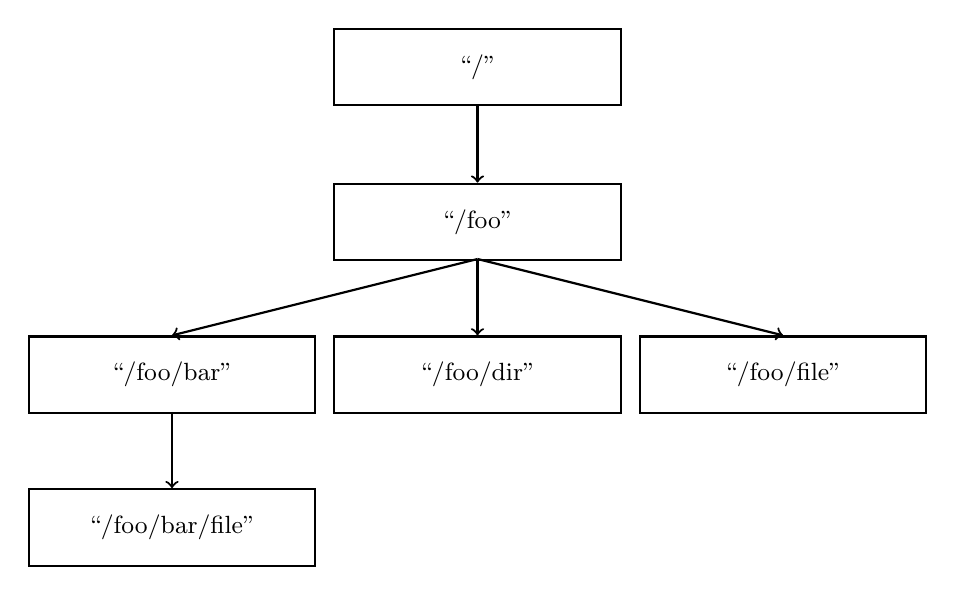
\begin{tikzpicture}{xscale=0.95,yscale=0.95}
            \draw[thick, ->] (0, .08\textwidth) -- (0, 0) node [anchor=north, rectangle, text centered, minimum height=.08\textwidth, minimum width=.3\textwidth, draw=black, font=\small] {``/foo/bar/file''};
            \draw[thick, ->] (.32\textwidth, .24\textwidth) -- (0, .16\textwidth) node [anchor=north, rectangle, text centered, minimum height=.08\textwidth, minimum width=.3\textwidth, draw=black, font=\small] {``/foo/bar''};
            \draw[thick, ->] (.32\textwidth, .24\textwidth) -- (.32\textwidth, .16\textwidth) node [anchor=north, rectangle, text centered, minimum height=.08\textwidth, minimum width=.3\textwidth, draw=black, font=\small] {``/foo/dir''};
            \draw[thick, ->] (.32\textwidth, .24\textwidth) -- (.64\textwidth, .16\textwidth) node [anchor=north, rectangle, text centered, minimum height=.08\textwidth, minimum width=.3\textwidth, draw=black, font=\small] {``/foo/file''};
            \draw[thick, ->] (.32\textwidth, .4\textwidth) -- (.32\textwidth, .32\textwidth) node [anchor=north, rectangle, text centered, minimum height=.08\textwidth, minimum width=.3\textwidth, draw=black, font=\small] {``/foo''};
            \node [anchor=south, rectangle, text centered, minimum height=.08\textwidth, minimum width=.3\textwidth, draw=black, thick, font=\small] at (.32\textwidth, .4\textwidth) {``/''};
        \end{tikzpicture}
        \caption{\label{subfig:FPI} Full-path indexing only keeps full-paths.}
    \end{subfigure}
    \begin{subfigure}[t]{.5\textwidth}
        \centering
        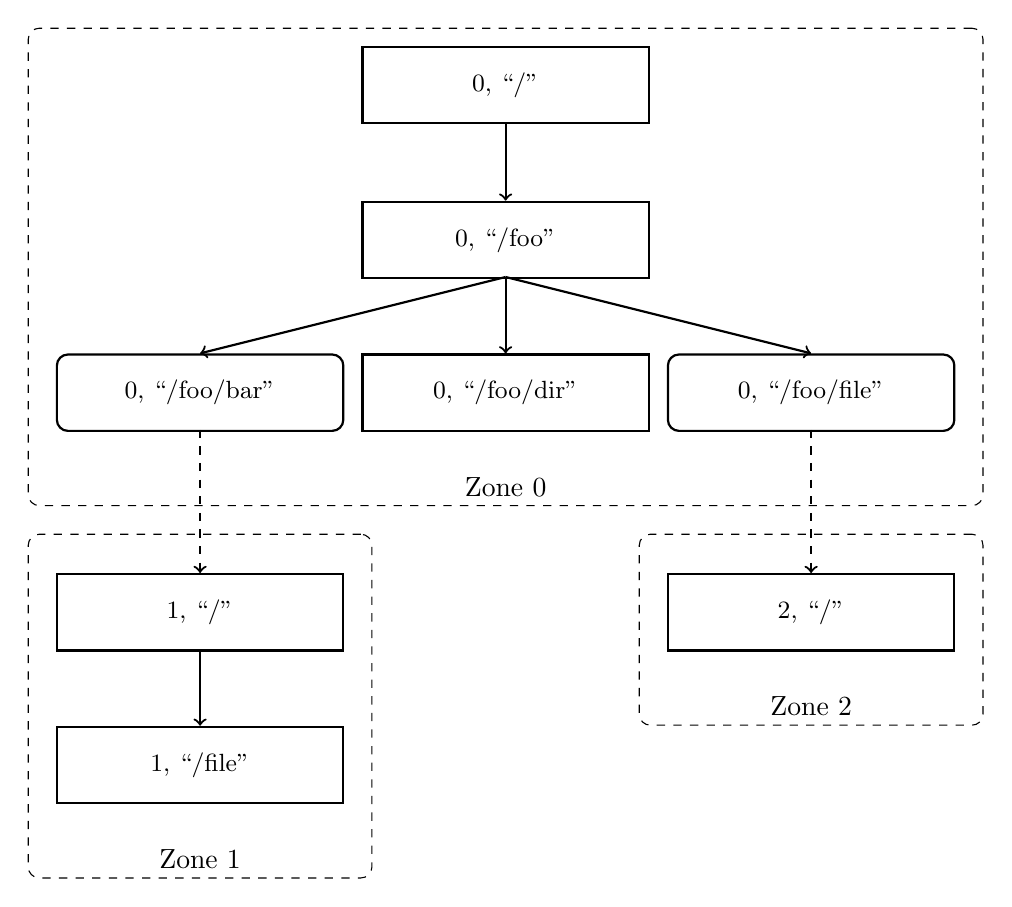
\begin{tikzpicture}{xscale=0.95,yscale=0.95}
            \node [anchor=south, rectangle, rounded corners, minimum height=.50\textwidth, minimum width=\textwidth, draw=black, dashed] at (.32\textwidth, 0) {};
            \node [anchor=south] at (.32\textwidth, 0) {Zone 0};
            \draw[thick, ->] (.32\textwidth, .24\textwidth) -- (0, .16\textwidth) node [anchor=north, rectangle, rounded corners, text centered, minimum height=.08\textwidth, minimum width=.3\textwidth, draw=black, font=\small] {0, ``/foo/bar''};
            \draw[thick, ->] (.32\textwidth, .24\textwidth) -- (.32\textwidth, .16\textwidth) node [anchor=north, rectangle, text centered, minimum height=.08\textwidth, minimum width=.3\textwidth, draw=black, font=\small] {0, ``/foo/dir''};
            \draw[thick, ->] (.32\textwidth, .24\textwidth) -- (.64\textwidth, .16\textwidth) node [anchor=north, rectangle, rounded corners, text centered, minimum height=.08\textwidth, minimum width=.3\textwidth, draw=black, font=\small] {0, ``/foo/file''};
            \draw[thick, ->] (.32\textwidth, .4\textwidth) -- (.32\textwidth, .32\textwidth) node [anchor=north, rectangle, text centered, minimum height=.08\textwidth, minimum width=.3\textwidth, draw=black, font=\small] {0, ``/foo''};
            \node [anchor=south, rectangle, text centered, minimum height=.08\textwidth, minimum width=.3\textwidth, draw=black, thick, font=\small] at (.32\textwidth, .4\textwidth) {0, ``/''};
            \node [anchor=south, rectangle, rounded corners, minimum height=.36\textwidth, minimum width=.36\textwidth, draw=black, dashed] at (0, -.39\textwidth) {};
            \node [anchor=south] at (0, -.39\textwidth) {Zone 1};
            \node [anchor=north, rectangle, text centered, minimum height=.08\textwidth, minimum width=.3\textwidth, draw=black, thick, font=\small] at (0, -.07\textwidth) {1, ``/''};
            \draw[thick, ->] (0, -.15\textwidth) -- (0, -.23\textwidth) node [anchor=north, rectangle, text centered, minimum height=.08\textwidth, minimum width=.3\textwidth, draw=black, font=\small] {1, ``/file''};
            \node [anchor=south, rectangle, rounded corners, minimum height=.2\textwidth, minimum width=.36\textwidth, draw=black, dashed] at (.64\textwidth, -.23\textwidth) {};
            \node [anchor=south] at (.64\textwidth, -.23\textwidth) {Zone 2};
            \node [anchor=north, rectangle, text centered, minimum height=.08\textwidth, minimum width=.3\textwidth, draw=black, thick, font=\small] at (.64\textwidth, -.07\textwidth) {2, ``/''};
            \draw[thick, dashed, ->] (0, .08\textwidth) -- (0, -.07\textwidth);
            \draw[thick, dashed, ->] (.64\textwidth, .08\textwidth) -- (.64\textwidth, -.07\textwidth);
        \end{tikzpicture}
        \caption{\label{subfig:RPI} Relative-path indexing splits the directory tree into zones and
            uses indirection between zones.}
    \end{subfigure}
    \caption[Full-path indexing and relative-path indexing]{\label{fig:FPIRPI}
        The same directory tree under full-path indexing and relative-path indexing.}
\end{figure}

Relative-path-indexed \betrfs~\citep{betrfs2,betrfs2tos} backed away from
full-path indexing and introduced relative-path indexing,
which is also called zoning.
Relative-path indexing partitions the directory hierarchy into zones.
Each zone has a zone ID (the root zone always has zone ID 0), which is analogous
to an inode number, and a single root file or directory.
All file or directory in a zone is indexed relative to the zone root.
If the file or directory is the root of another zone, the entry contains the
zone ID to redirect queries.
With the introduction of zoning, each key in \betrfs contains two parts,
a zone ID and the relative path to the zone root.

Figure~\ref{fig:FPIRPI} shows an example of the same directory tree under
full-path indexing and relative-path indexing.
In Figure~\ref{subfig:RPI}, relative-path indexing partitions the directory
into three zones.
Zone 0 is the root zone, Zone 1 is rooted at a directory ``/foo/bar'' and
Zone 2 is rooted at a file ``/foo/file''.
When querying the key/value store for file ``/foo/file'' with key
(0, ``/foo/file''), the file system gets a special value that
indicates the entry is the root of Zone 2.
Subsequently, the file system queries the key/value store with key (2, ``/'')
and gets the correct value.
Similarly, the file system notices the key for directory ``/foo/bar'' is
(3, ``/'').
Therefore, when querying for file ``/foo/bar/file'', it uses key (3, ``/file'').

Relative-path indexing tries to balance locality and rename performance through
a target zone size.
On one hand, full-path indexing is still maintained within a zone,
so larger zone size gives better locality.
On the other hand, smaller zone size imposes a lower bound on rename cost,
because no rename needs to mutate more key/value pairs than the zone size.
Relative-path-indexing with an infinite zone size is equivalent to
full-path-indexing, while relative-path-indexing with a zero zone size is the
same as indexing with inode numbers.

Relative-path indexing keeps zones within the target zone size by zone splits
and merges.
In particular, for each file or directory, \betrfs keeps a counter in its inode
to indicate how many key/value pairs will be affected if the file or directory
is renamed.
When the counter of a directory or file becomes too big,
relative-path indexing moves it to its own zone with a zone split,
updating all affected keys with the new zone ID and relative-paths.
When the counter of a zone root becomes too small (1/4 of the maximum
size), relative-path indexing merges it to the parent zone.

\begin{figure}[t]
    \centering
    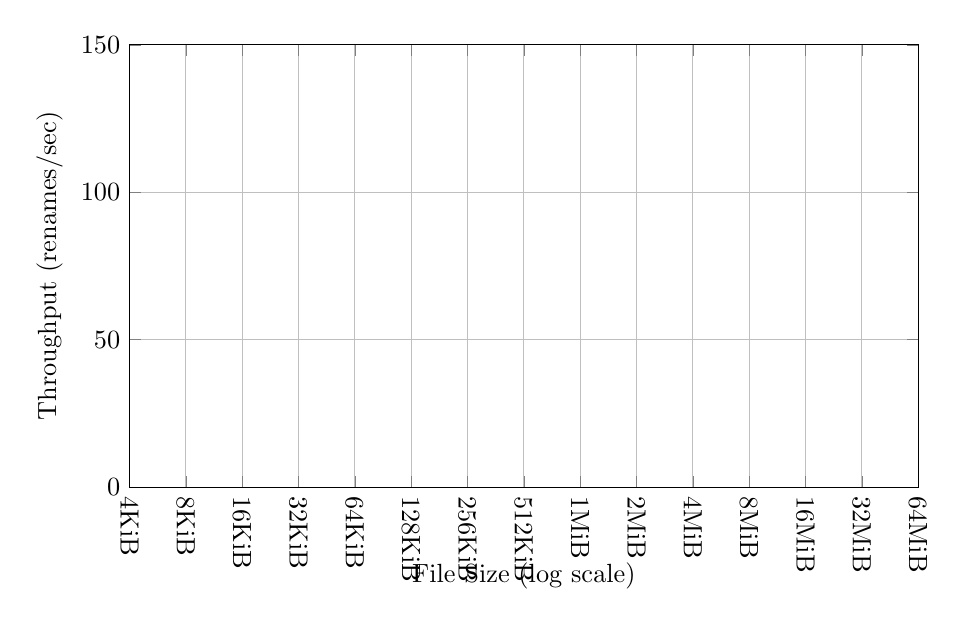
\begin{tikzpicture}[yscale=0.95, xscale=0.95]
        \begin{axis}[
                xlabel={File Size (log scale)},
                x label style={at={(axis description cs:0.5,-0.15)},anchor=north},
                ylabel={Throughput (renames/sec)},
                xmin=12,
                xmax=26,
                xtick={12,13,14,15,16,17,18,19,20,21,22,23,24,25,26},
                xticklabels={4KiB,8KiB,16KiB,32KiB,64KiB,128KiB,256KiB,512KiB,1MiB,2MiB,4MiB,8MiB,16MiB,32MiB,64MiB},
                xticklabel style={rotate=270, anchor=west},
                ymin=0,
                ymax=150,
                grid=major,
                scaled x ticks=false,
                scaled y ticks=false,
                legend columns=4,
                legend cell align=left,
                height=.618\linewidth,
                width=\linewidth,
            ]
            \addFileRenamePlot{ext4};
            \addFileRenamePlot{btrfs};
            \addFileRenamePlot{xfs};
            \addFileRenamePlot{zfs};
            \addFileRenamePlot{nilfs2};
            \addFileRenamePlot{betrfs3};
            \addFileRenamePlot{betrfs3-max};
        \end{axis}
    \end{tikzpicture}
    \caption[The performance of file renames in relative-path-indexed file systems]{\label{fig:file_rename_rpi}
        Throughput of renaming a file of different sizes (higher is better).
        The performance of relative-path-indexed \betrfsThree doesn't
        degrade when the file being renamed becomes larger.}
\end{figure}

The implementation of relative-path-indexed \betrfs, \betrfsTwo, adopts a
512KiB default zone size.
This default zone size is small enough that renames on \betrfsTwo are almost
as fast as on inode-based file systems.
At the same time, the default zone size is large enough that directory
traversals are almost as fast as \betrfsOne.

Figure~\ref{fig:file_rename_rpi} shows the results of running the file rename
benchmark on \betrfsThree (\betrfsThree is \betrfsTwo with some bug fixes).
The benchmark renames a file of different sizes 100 times, each followed by a
\texttt{fsync} of the parent directory.
We run the benchmark on \betrfsThree twice,
one on \betrfsThree (with the default zone size),
the other on full-path-indexed \betrfsThree,
that is, \betrfsThree with an infinite zone size.
As shown in the graph, before reaching the target zone size, 512KiB,
the performance of relative-path-indexed \betrfsThree is similar to
full-path-indexed \betrfsThree.
However, when the file size reaches the target zone size, the file forms its
own zone and file renames become pointer swings.
Therefore, after the target zone size,
the performance of file renames in relative-path-indexed \betrfsThree
doesn't degrade when the file size becomes larger.

\begin{table}[t]
    \centering
    \begin{tabular}{l|.@{${}\pm{}$}.}
    \hline
    File system & \multicolumn{2}{c}{grep (sec)}  \\
    \hline
    \hline
    \pgfkeysvalueof{/fs-names/ext4}        &  37.795 &  1.145 \\
    \pgfkeysvalueof{/fs-names/btrfs}       &   9.265 &  0.139 \\
    \pgfkeysvalueof{/fs-names/xfs}         &  48.130 &  0.206 \\
    \pgfkeysvalueof{/fs-names/zfs}         & 463.184 & 33.878 \\
    \pgfkeysvalueof{/fs-names/nilfs2}      &   8.318 &  0.107 \\
    \pgfkeysvalueof{/fs-names/betrfs3}     &   5.070 &  0.078 \\
    \pgfkeysvalueof{/fs-names/betrfs3-max} &   4.022 &  0.055 \\
    \hline
    \end{tabular}
    \caption[The performnace of directory traversals in relative-path-indexed file systems]{\label{tab:dir_ops_rpi}
        Time to perform recursive grep of the Linux source directory (lower is better).
        The performance of relative-path-indexed \betrfsThree is still better than
        conventional file systems.}
\end{table}

Table~\ref{tab:dir_ops_rpi} shows the performance of directory traversals on
different file systems.
The benchmark measures the time to \texttt{grep} the  Linux 3.11.10 source
directory.
Relative-path-indexed \betrfsThree is slightly slower than full-path-indexed
\betrfsThree, but still faster than other file systems.

\begin{figure}[t]
    \centering
    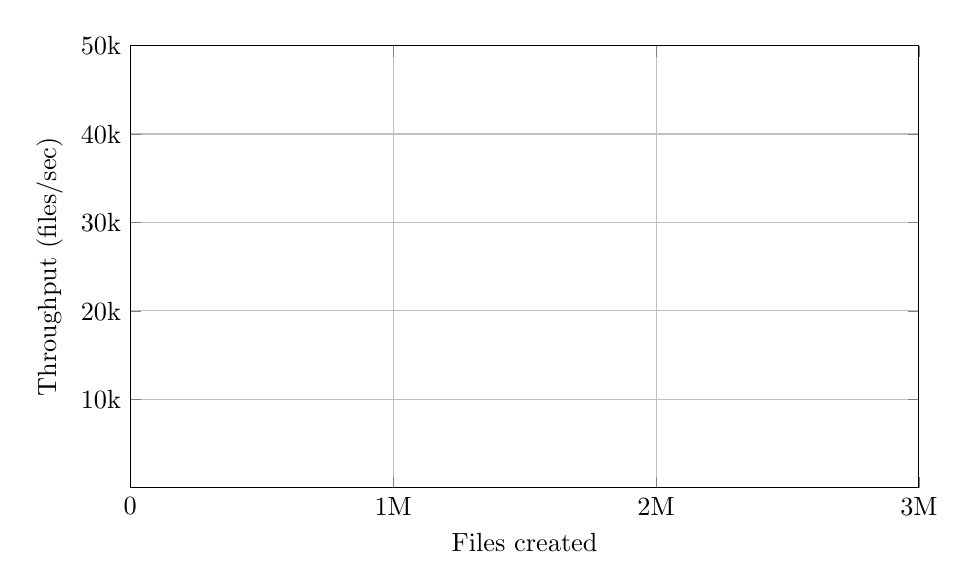
\begin{tikzpicture}[yscale=0.95,xscale=0.95]
        \begin{axis}[
            xlabel={Files created},
            ylabel={Throughput (files/sec)},
            xmin=0,
            xmax=3000000,
            ymin=10,
            ymax=50000,
            mark repeat=10,
            xtick={0,1000000,2000000,3000000},
            xticklabels={0,1M,2M,3M},
            ytick={10000,20000,30000,40000,50000},
            yticklabels={10k,20k,30k,40k,50k},
            grid=major,
            scaled x ticks=false,
            scaled y ticks=false,
            legend cell align=left,
            transpose legend,
            height=.618\linewidth,
            width=\linewidth,
        ]
        \addTokubenchPlot{betrfs3};
        \addTokubenchPlot{betrfs3-max};
        \end{axis}
    \end{tikzpicture}
    \caption[Zone maintainance cost in TokuBench benchmark]{
        Cumulative file creation throughput during the Tokubench benchmark (higher is better).
        Compared to full-path-indexed \betrfsThree,
        relative-path-indexed \betrfsThree has a sudden
        performance drop because of zone splits.}
    \label{fig:tokuzone}
\end{figure}

However, relative-path indexing imposes zone maintenance costs on other file
system operations.
When a file system operation happens to trigger a zone split or merge,
in addition to the costs of the operation itself,
relative-path indexing charges the zone split or merge to that operations.
For instance, Figure~\ref{fig:tokuzone} shows the results of running Tokubench,
which creates 3 million small files in a balanced tree structure,
on \betrfsThree.
On the graph, two-thirds of the way through the TokuBench benchmark,
\betrfsThree with the default zone size shows a sudden,
precipitous drop in cumulative throughput for small file creation,
because the file system performs a huge amount of zone splits.
At that moment, all benchmarking directories are one file less than the target
zone size.
Therefore, creating one file in a directory results in a zone split,
updating all key/value pairs under the directory.
On the contrary, \betrfsThree with an infinite zone size
has a smooth curve throughout the benchmark
because no zone split happens with a infinite zone size.

Furthermore, relative-path indexing has bad worst-case performance.
It is possible to construct arrangements of nested directories that will each
reside in their own zone.
Reading a file in the deepest directory will require reading one zone per
directory (each with its own I/O),
essentially making the file system inode-based.
Such a pathological worst case is not possible with full-path indexing in a
\bet, and an important design goal for \betrfs is keeping a reasonable bound on
the worst cases.

Finally, relative-path indexing breaks the clean mapping of directory subtrees
onto contiguous ranges of the key space,
preventing us from using range-messages to implement bulk operations on entire
directory.
For example, with full-path indexing, we can use range-delete messages not
only to delete files, but an entire directory.
We could also use range messages to perform a variety of other operations on
the whole directory, such as recursive \texttt{chmod}, \texttt{chown} and
timestamp updates.
And, as we will eventually see with the range-clone operations, we can clone the
whole directory with one operation.

\section{Implementation}
\label{sec:bg:impl}

This section discusses implementation details of \fti.

\subsection{Synchronization}
\label{sec:bg:impl:sync}

\Fti maintains a readers-writer lock for each \bet node to synchronize
operations in the \bet.
In \fti, a query grabs the read locks of all nodes along the root-to-leaf path,
while a write operation grabs the write lock of the root node.
A node split or merge grabs the write locks of the parents and children
involved in the rebalancing process.
Similarly, the flushing process write-locks the parent and the child.

\subsection{The message buffer}
\label{sec:bg:impl:partition}

\Fti stores messages in a non-leaf node in multiple buffers, called partitions,
rather than keeping them in a single large buffer.
A non-leaf node in \fti with $n$ children has $n$ partitions, each corresponds
to a child of the node, and each partition stores messages in a list, sorted
by the logical timestamps.
When a message is injected or flushed to a non-leaf node, it is placed at the
tail of the list in the partition
that corresponds to the child the message will be flushed to later.

Such a design makes implementation simple.
\Fti keeps bookkeeping information for each partition and can
quickly figure out which child can receive the most messages
in the flushing process.
Also, because messages are sorted in the timestamp order, the flushing process
can simply iterate the list in the parent partition.
Moreover, a query doesn't need to fetch the whole non-leaf node,
because only one partition can contain messages with the query key.
Therefore, the amount of I/Os a query needs to perform is reduced.

A node split also needs to split the parent partition into two
new partitions, each for one child generated by the node split.
However, splitting a partition with messages is difficult because messages are
sorted by the timestamp order, instead of the key order.
Therefore, before splitting the child, the node split flushes all messages in
the parent partition to the child, emptying the parent partition.
Because a node split holds the write locks of the parent and the child,
no message can be injected into the parent partition
before the node split completes.
And flushing messages in a node split doesn't incur additional I/Os
since the node split fetches and dirties the parent and the child anyway.
Similarly, a node merge also flushes the parent partitions to the children being
merged.

\subsection{Transactions}
\label{sec:bg:impl:txn}

\Fti performs multiple operations atomically in transactions.
To avoid transactions from touching the same key, \fti maintains locks for key
ranges in an interval tree.
Before querying a key, the operation should read-lock the specific key range so
that no other transaction can modify keys in the key range.
Likewise, before modifying a key, the operation should write-lock the specific
key range.
The key locks are released only when the transaction commits or aborts.
When a transaction fails to lock a key range for its operation, it should
abort.

Transaction commits or aborts are implemented with transaction-commit or
transaction-abort messages.
When a transaction commits or aborts, it injects one transaction-commit or
transaction-abort message for each operation it performs.
For example, consider an insert for key $k$ in a transaction.
During the transaction, the insert injects an \putm message with key $k$
to the lifted \bet.
When the transaction commits, the transaction injects a transaction-commit
message with key $k$ for the insert, finalizing the insert.
If the transaction aborts, the transaction injects a transaction-abort message
with key $k$ for the insert, invalidating the insert.
Queries need to ignore uncommitted or aborted messages.

\subsection{Recovery}
\label{sec:bg:impl:recover}

\Fti ensures crash consistency by keeping a redo log of pending messages and
applying messages to \betrfs nodes with copy-on-write.
At periodic intervals (60 seconds in \betrfs), \fti checkpoints its lifted
\bets by writing all dirty nodes to the disk.
Then, \fti can discards the redo log that stores operations after previous
checkpoint.
Application can ensure all changes are persistent on the disk by force a log
flush.
When a machine fails, after rebooting, \fti simply replays the redo log on the
lifted \bets at the last checkpoint.

\section{Conclusion}

\betrfs is a general file system designed for all operations, with a particular
focus on random writes and locality.
The underlying data structure, \bets, performs random writes much faster than
\btrees by cascading writes in batches.
The full-path indexing schema of \betrfsOne ensures good locality.
However, the preliminary implementation of namespace operations in \betrfsOne
is slow because they need to iterate all affected keys.
The relative-path indexing schema of \betrfsTwo enables fast renames by bounding
the maximum number of affected in a rename.
However, it imposes zone maintenance costs on other file system operations.
Also, it breaks the full-path indexing, preventing us from implementing other
efficient namespace operations that are difficult on other file systems.

